\chapter{RESULTS AND EVALUATION}
\label{chap:evalution}

\section{Evaluation Methods}

The evaluation process is conducted through two main metrics: Mean Opinion Scores (MOS) and Fréchet Inception Distance (FID).

\subsection{Evaluation Based on Human Perception}

\subsubsection{Mean Opinion Scores (MOS)}

Currently, there is no standard metric for gesture generation, especially for gesture generation from speech. Therefore, this thesis relies on subjective human evaluation to conduct experimental assessments. 
Similar to previous methods \cite{yoon2022genea}, \cite{kucherenko2021large}, speech-driven gesture generation models still lack objective metrics that consistently reflect human subjective perception \cite{alexanderson2022listen}.

MOS is measured through three criteria:

\begin{itemize}
	\item Human-likeness
	\item Gesture-Speech Appropriateness
	\item Gesture-Style Appropriateness
\end{itemize}

One of the contributions of this thesis is the development of the \hyperlink{https://genea-workshop.github.io/leaderboard/}{GENEA Leaderboard} \footnote{ \url{https://genea-workshop.github.io/leaderboard} } \cite{nagy2024towards}. This system includes HEMVIP (\textbf{H}uman \textbf{E}valuation of \textbf{M}ultiple \textbf{V}ideos in \textbf{P}arallel), which is used to compare visual generation results between videos rendered by different models.

\begin{figure}[H]
	\centering
	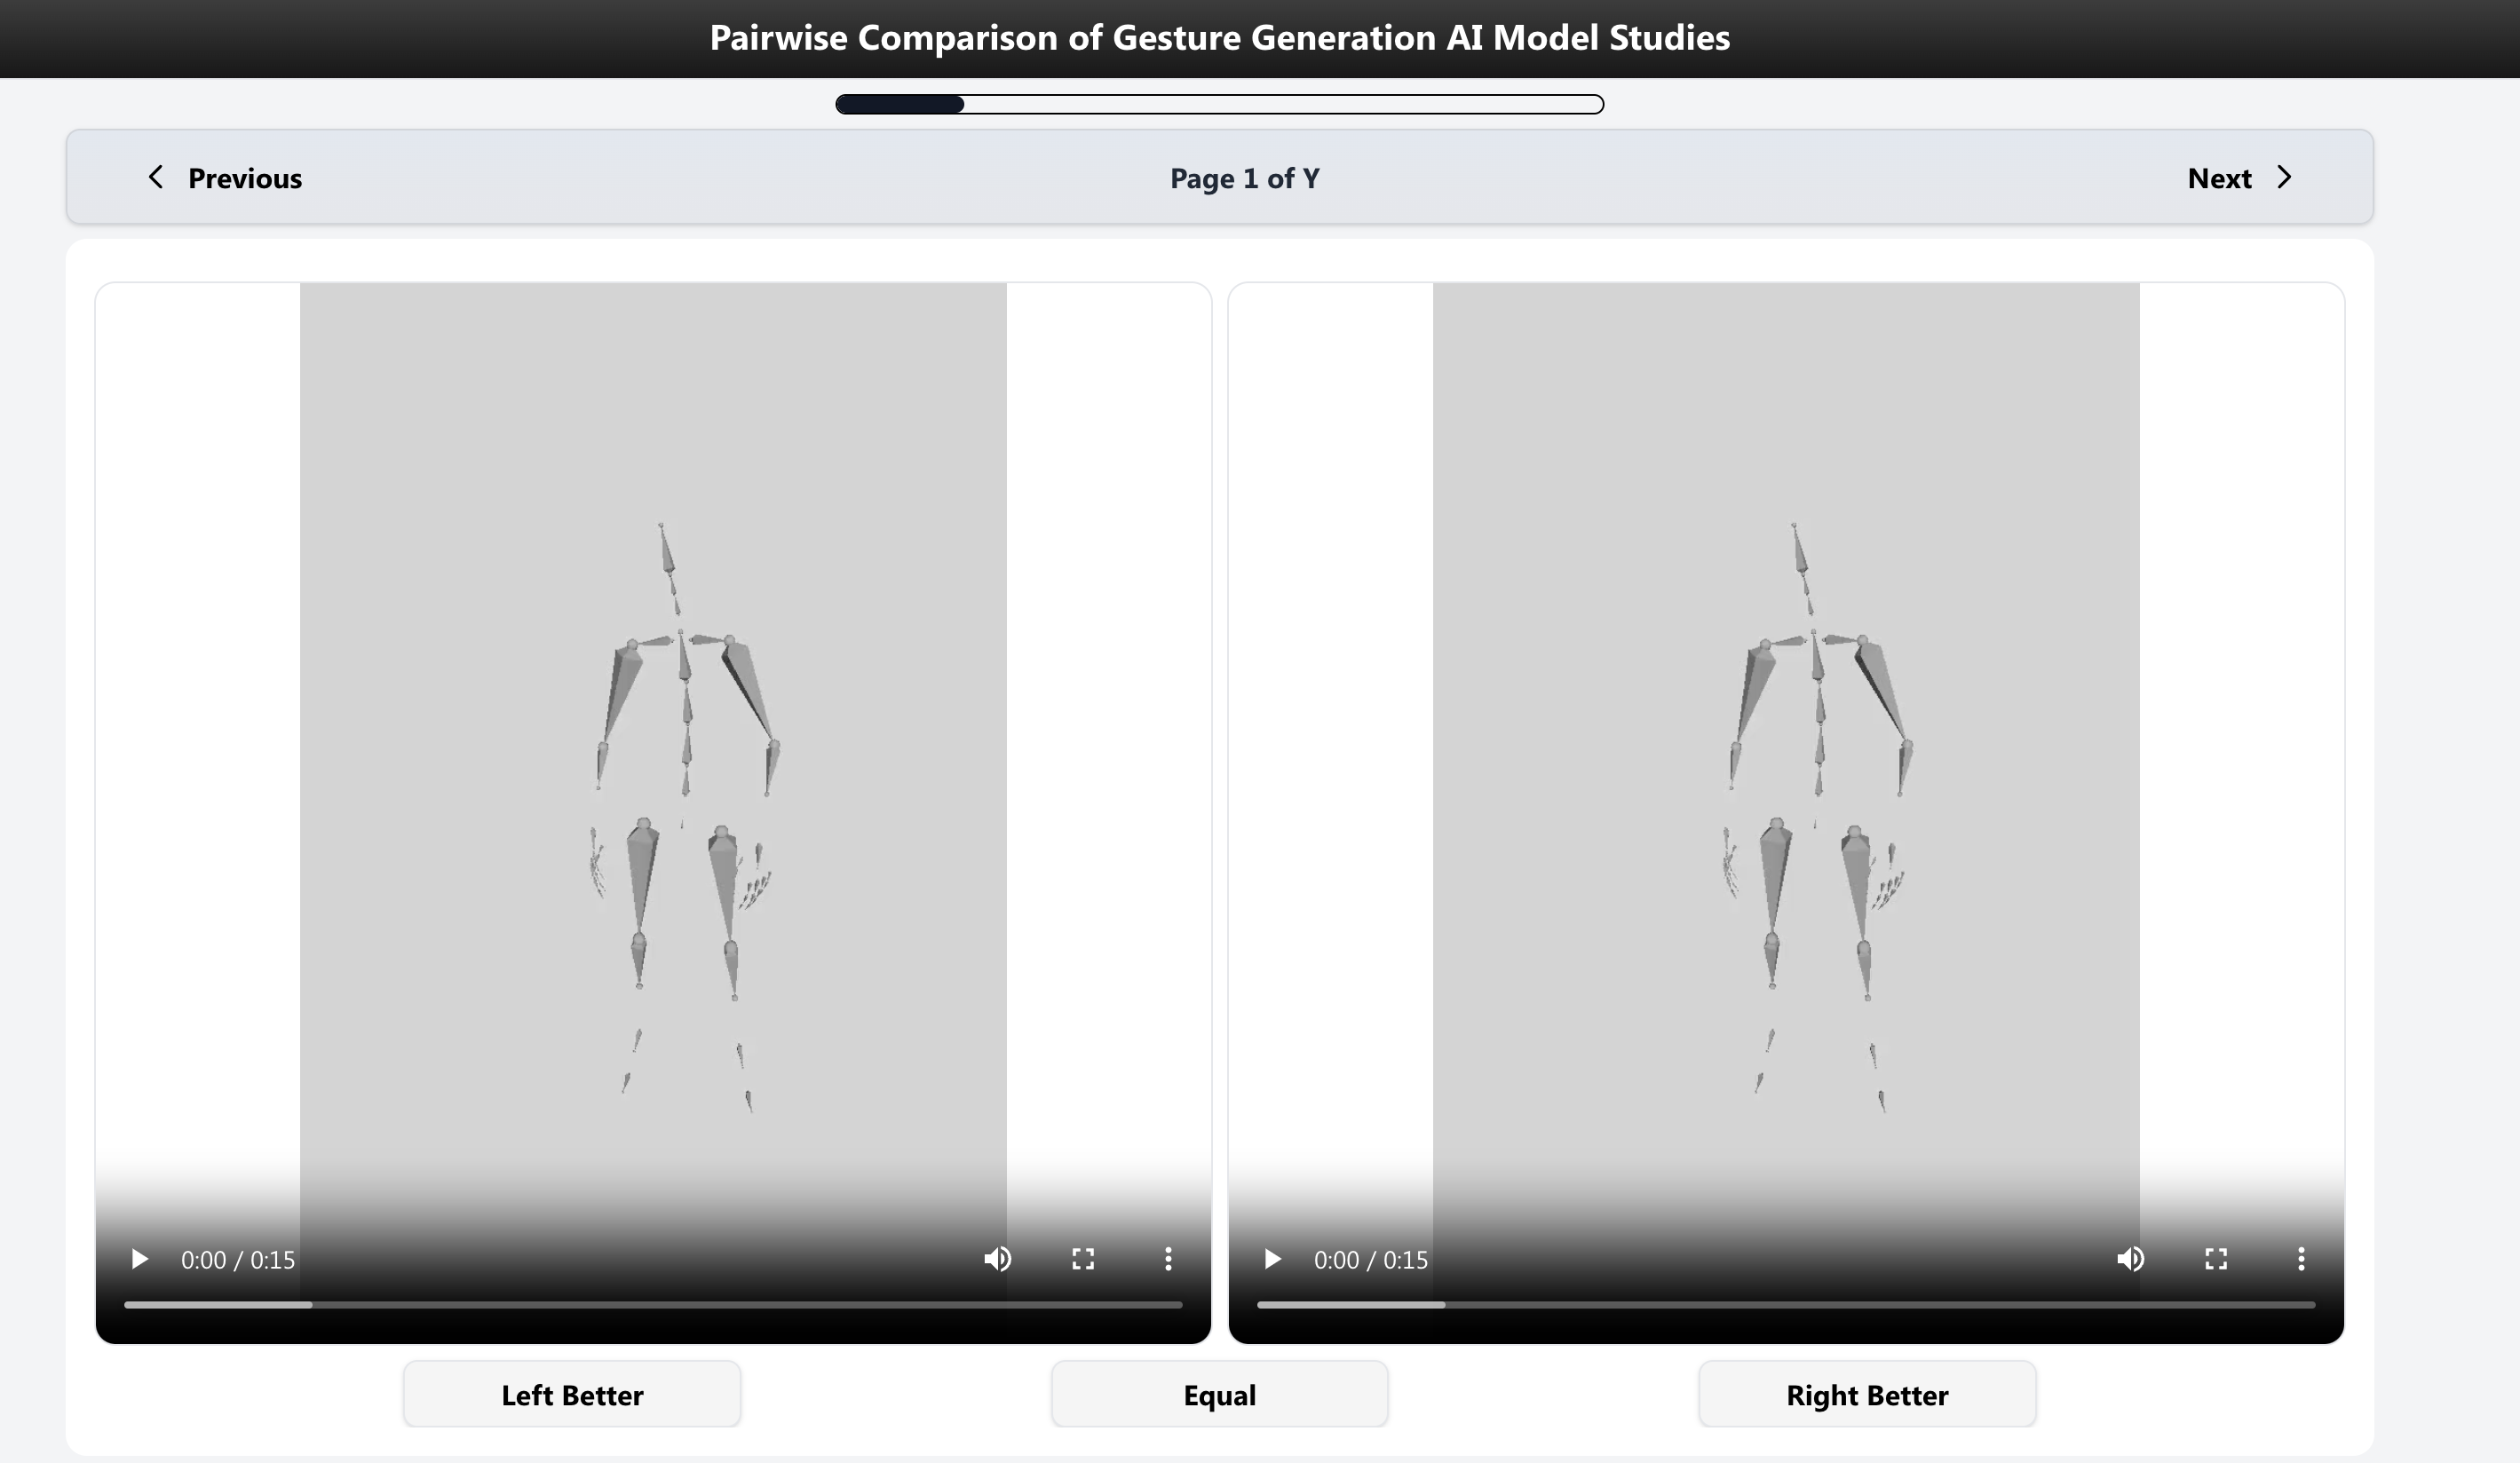
\includegraphics[width=\textwidth]{hemvip}
	\caption{HEMVIP system used to evaluate rendering results of two models}
\end{figure}

Within the GENEA group (\textbf{G}eneration and \textbf{E}valuation of \textbf{N}on-verbal Behaviour for \textbf{E}mbodied \textbf{A}gents), we hire evaluators on Prolific and conduct a user study based on the rendered video results. Participants rate the results as \textit{Left Better}, \textit{Equal}, or \textit{Right Better}. The updated scores are $-1$, $0$, and $1$ for each model, including ground truth data. The comparative results for all models are updated using the Elo rating system.

The source code of the program is available at \hyperlink{https://github.com/hemvip/hemvip.github.io/}{github.com/hemvip.github.io}
\footnote{HEMVIP 2 \url{https://github.com/hemvip/hemvip.github.io}}.

\subsection{Evaluation Based on Quantitative Metrics}

\subsubsection{Mean Square Error (MSE)}

The mean square error between the predicted gesture sequence $\hat{\mathbf{y}}_i^{1:M \times D}$ and the ground-truth gesture sequence $\mathbf{y}_i^{1:M \times D}$ is computed as follows:

\begin{equation}
\text{MSE} = \frac{1}{n} \sum_{i=1}^n \left\| \mathbf{y}_i^{1:M \times D} - \hat{\mathbf{y}}_i^{1:M \times D} \right\|^2
\end{equation}

Where:
\begin{itemize}
	\item $n$ is the number of data samples.
	\item $\mathbf{y}_i^{1:M \times D}$ is the ground truth of the $i^{th}$ sample, with $M$ being the number of frames and $D$ the number of data dimensions.
	\item $\hat{\mathbf{y}}_i^{1:M \times D}$ is the predicted value of the $i^{th}$ sample, having the same size $M \times D$.
	\item $\left\| \mathbf{y}_i^{1:M \times D} - \hat{\mathbf{y}}_i^{1:M \times D} \right\|^2$ is the squared norm of the difference between the ground truth and the predicted matrix.
\end{itemize}

MSE measures the average squared difference between the actual and predicted gesture sequences. The smaller the value, the more accurate the model's predictions. Evaluation results are presented in \autoref{subsec:MSEResult}.

\subsubsection{Fréchet Gesture Distance (FGD)}

Similar to image generation methods that use the Fréchet Inception Distance (FID) to measure distributional differences between real and generated data, the Fréchet Gesture Distance (FGD) measures the similarity in distribution between generated gesture sequences $\hat{\mathbf{y}}_i^{1:M \times D}$ and real gesture sequences $\mathbf{y}_i^{1:M \times D}$:

\begin{equation}
	\text{FGD} = \left\| \hat{\mu} - \mu \right\|^2 + \operatorname{Tr}\left( \Sigma + \hat{\Sigma} - 2 \sqrt{\Sigma \hat{\Sigma}} \right)
	\label{eq:fidscore}
\end{equation}

Where $n$ is the number of samples, and the parameters are defined as:

\begin{itemize}
	\item $\mu = \frac{1}{n} \sum_{i=1}^n \mathbf{y}_i^{1:M \times D}$ and $\hat{\mu} = \frac{1}{n} \sum_{i=1}^n \hat{\mathbf{y}}_i^{1:M \times D}$ are the mean feature vectors of the real dataset $\mathbf{y}_i^{1:M \times D}$ and generated dataset $\hat{\mathbf{y}}_i^{1:M \times D}$, respectively.
	 
	\item $\Sigma = \frac{1}{n-1} \sum_{i=1}^n \left( \mathbf{y}_i^{1:M \times D} - \mu \right) \left( \mathbf{y}_i^{1:M \times D} - \mu \right)^T$ and
	
	$\hat{\Sigma} = \frac{1}{n-1} \sum_{i=1}^n \left( \hat{\mathbf{y}}_i^{1:M \times D} - \hat{\mu} \right) \left( \hat{\mathbf{y}}_i^{1:M \times D} - \hat{\mu} \right)^T$ are the covariance matrices of the features from the real and generated datasets, respectively.
	
	\item $\operatorname{Tr}(\cdot)$ denotes the matrix trace operator, which sums the diagonal elements.
	
	\item $\sqrt{\Sigma \hat{\Sigma}}$ denotes the matrix square root of the product of the two covariance matrices.
\end{itemize}

A low FGD score indicates that the distribution of generated gestures is close to the real gestures, while a high FGD suggests a large distributional difference and therefore lower gesture generation quality. In this thesis, the evaluation is performed on the predicted gesture sequence $\hat{\mathbf{x}}^{0} \in \mathbb{R}^{1:M \times D}$ and the ground-truth gesture sequence $\mathbf{x}_{0} \in \mathbb{R}^{1:M \times D}$.

\section{Evaluation Results}
\label{sec:result}

\subsection{User Study Evaluation Results}

\subsubsection{MOS Evaluation Results}

This thesis reuses the evaluation results of the baseline model \textbf{DiffuseStyleGesture} \cite{yang2023diffusestylegesture} for human perception metrics, as gesture generation remains a nascent field and the cost of evaluating multiple models is high. Therefore, this thesis does not include evaluation results for the proposed \textbf{OHGesture} model.

\begin{figure}[htbp]
	\centering
	\begin{subfigure}[b]{0.3\textwidth}
		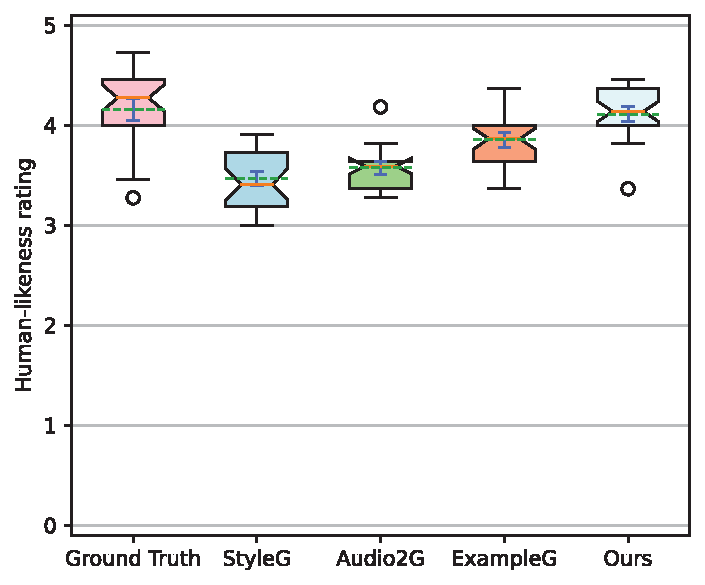
\includegraphics[width=\textwidth]{BoxHumanLikeness.pdf}
		\caption*{(a) Human-likeness}
	\end{subfigure}
	\hfill
	\begin{subfigure}[b]{0.3\textwidth}
		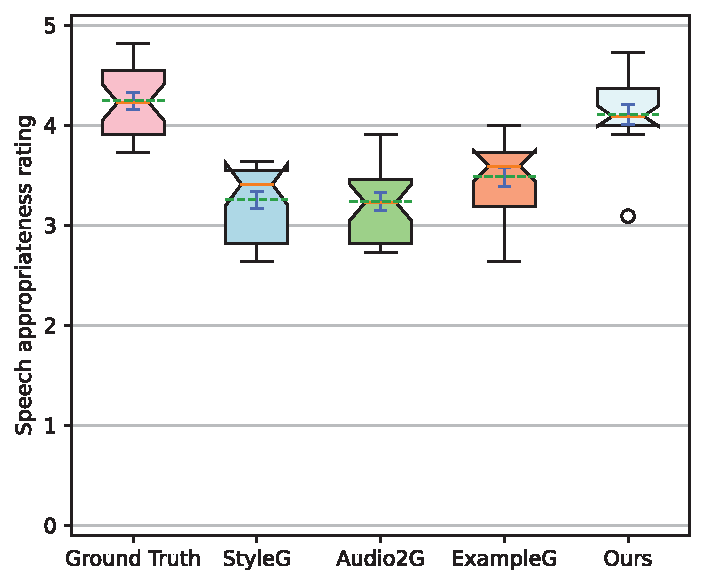
\includegraphics[width=\textwidth]{BoxSpeechAppropriateness.pdf}
		\caption*{\small (b) Speech Appropriateness}
	\end{subfigure}
	\hfill
	\begin{subfigure}[b]{0.3\textwidth}
		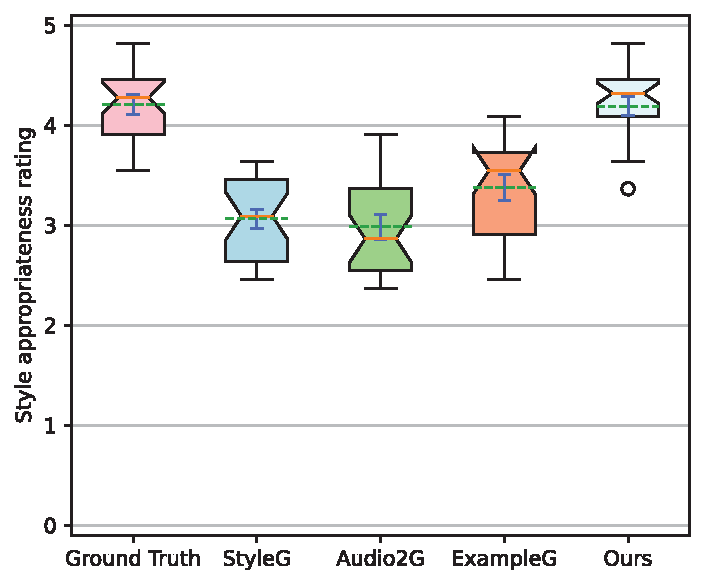
\includegraphics[width=\textwidth]{BoxStyleAppropriateness.pdf}
		\caption*{(c) Style Appropriateness}
	\end{subfigure}
	
	\label{fig:compare }
\end{figure}

To understand the visual performance of the proposed method, this thesis conducts a user study comparing gestures generated by the proposed method with those from real motion capture data. The duration of the evaluated video clips ranges from 11 to 51 seconds, with an average length of 31.6 seconds — longer than clips used in the GENEA evaluation \cite{yoon2022genea} (8–10 seconds), as longer durations can provide clearer and more convincing results \cite{yang2022reprgesture}. Participants rated each video on a scale from 5 to 1, labeled $\texttt{excellent}$, $\texttt{good}$, $\texttt{fair}$, $\texttt{poor}$, and $\texttt{bad}$. 

\begin{table}[H]
	\centering
	\begin{tabular}{lcc}
		\hline
		\multicolumn{1}{c}{Name} &
		\begin{tabular}[c]{@{}c@{}}Human\\ likeness \end{tabular}$\uparrow$ &
		\begin{tabular}[c]{@{}c@{}}Gesture-speech\\ appropriateness\end{tabular}$\uparrow$ \\ \hline
		Ground Truth          & 4.15 $\pm$ 0.11          & 4.25 $\pm$ 0.09          \\
		Ours                  & \textbf{4.11 $\pm$ 0.08} & \textbf{4.11 $\pm$ 0.10} \\
		\quad$-$ WavLM             & 4.05 $\pm$ 0.10          & 3.91 $\pm$ 0.11          \\
		\quad$-$ Cross-local attention   & 3.76 $\pm$ 0.09          & 3.51 $\pm$ 0.15          \\
		\quad$-$ Self-attention    & 3.55 $\pm$ 0.13          & 3.08 $\pm$ 0.10          \\
		\quad$-$ Attention + GRU&
		3.10 $\pm$ 0.11 &
		2.98 $\pm$ 0.14 \\
		\quad$+$ Forward attention & 3.75 $\pm$ 0.15          & 3.23 $\pm$ 0.24          \\
		\hline
	\end{tabular}
	\caption{Evaluation results using MOS}
	\label{table:MOSScore}
\end{table}
% Results of the ablation studies. "$-$" indicates removed modules, "$+$" indicates added modules. Bold indicates best performance.

\subsection{Quantitative Evaluation Results}

\subsubsection{Evaluation Results using MSE}
\label{subsec:MSEResult}

In this thesis, the predicted gesture sequence is segmented over $M$ frames. Mean Square Error (MSE) is applied to the gesture sequence $\mathbf{x}^{1:M \times D}$.

\begin{table}[H]
	\centering
	\resizebox{\textwidth}{!}{%
		\begin{tabular}{lcccccc}
			\hline
			\multicolumn{1}{c}{Emotion} & Neutral & Sad & Happy & Relaxed & Elderly & Angry \\ \hline
			DiffuseStyleGesture  & 75.04 & 51.40 & 110.18 & 130.83     & 116.03    & 78.53     \\
			ZeroEGG & 136.33 & 81.22 & 290.47 & 140.24     & 102.44    & 181.07     \\
			\hline
			Proposed Model                     &         &         &         &           &          &                 \\
			\quad \textbf{OHGesture} & 161.22 & 89.58 & 279.95 & 156.93   & 99.86   & 215.24    \\
			\hline
		\end{tabular}%
	}
	\caption{Mean Square Error results across 6 emotion categories}
	\label{table:EvaluationMSE}
\end{table}

\subsubsection{Evaluation Results using FGD}

This thesis proposes Fréchet Gesture Distance (FGD), a gesture-based variant of FID, and develops the open-source tool \hyperlink{https://github.com/GestureScore/GestureScore}{GestureScore} \footnote{Github/GestureScore: \url{https://github.com/GestureScore/GestureScore}}. In GestureScore, an Inception V3 model is implemented to encode the frame sequence $\bx^{1:M \times D}$ into a latent feature vector of size $32 \times 32$, which is then used as input to \autoref{eq:fidscore}. The following \autoref{table:EvalFGD} shows the FGD evaluation results of the OHGesture model using GestureScore.

\begin{table}[H]
	\centering
	\begin{tabular}{lcc}
		\hline
		\multicolumn{1}{c}{Name} & FGD on Feature Vectors & \begin{tabular}[c]{@{}c@{}} FGD on Raw Data \end{tabular} \\ \hline
		Ground Truth             & -       & -          \\
		Ours                     &       & \\
		\quad OHGesture (Feature D=1141) & 2.058      & 9465.546 \\
		\quad OHGesture (Rotations) & 3.513       & 9519.129 \\
		\hline
	\end{tabular}
	\caption{Evaluation results of Fréchet Gesture Distance (FGD) on $\bx^{1:M \times D}$ (from frame 1 to frame M, with D features per frame)}
	\label{table:EvalFGD}
\end{table}

\begin{itemize}[]
	\item \textbf{Feature Vectors:} The BVH files are used to convert the entire skeleton of each frame into a feature vector of size $D = 1141$, as described in \autoref{eq:gesturevector}.
	
	\item \textbf{Rotations:} From the resulting BVH file, this thesis extracts the rotation angles, $D = 225$ ($225 = 75 \times 3$), from the gesture sequence of length $M$ frames for evaluation in the OHGesture row below.
\end{itemize}

\section{Building and Standardizing a Gesture Generation Evaluation System}

Currently, gesture generation is an active research area with many different models. However, there is no shared evaluation metric. Traditional metrics such as FID (Fréchet Inception Distance) or IS (Inception Score) fail to capture the human-likeness, speech appropriateness, and style appropriateness of generated gestures. Moreover, models are trained and evaluated on different datasets, making it difficult to compare results and determine which model is superior or state-of-the-art. This lack of a standardized evaluation protocol hampers progress in gesture generation research.

To address this, the thesis proposes building an online leaderboard system \cite{nagy2024towards} \hyperlink{https://genea-workshop.github.io/leaderboard/}{GENEA Leaderboard} \footnote{GENEA Leaderboard: \url{https://genea-workshop.github.io/leaderboard/}}, which ranks gesture generation models. The thesis collects and processes gesture data from multiple languages and datasets, standardizes them into a unified dataset, and invites authors of various models to train and infer on this standardized set. The resulting generated gestures are then evaluated by hired participants through Prolific. 

The thesis is also building an online system \hyperlink{https://github.com/hemvip/hemvip.github.io}{hemvip/hemvip.github.io} \footnote{HEMVIP2 \url{https://github.com/hemvip/hemvip.github.io}} to support the evaluation process via Prolific-based crowd-sourcing. Evaluation results for the OHGesture model will be added based on this system.

Through this evaluation system, the research aims to establish a common benchmark, thereby fostering advancement in gesture generation.
